% ============================================================
\section{Results}
\label{sec:results}
% ============================================================

We report results in the order in which they bear on the central claims, and we lead
with the locked out-of-sample test rather than the in-sample fit. The first block
covers test-window and full-period performance against the benchmark panel
(Section~\ref{sec:res_oos}) and the spanning-alpha evidence
(Section~\ref{sec:res_alpha}), followed by robustness to known risk factors and to the
parameter search (Section~\ref{sec:res_factors}) and the comparison of the
minimum-correlation rule against optimised portfolio-construction alternatives
(Section~\ref{sec:res_construction}). Only then do we turn inward: the in-sample rule
attribution (Section~\ref{sec:res_insample}), the nested per-rule ladder
(Section~\ref{sec:res_ladder}), the risk-control role of minimum correlation
(Section~\ref{sec:res_mincorr}), robustness to transaction costs
(Section~\ref{sec:res_costs}), after-tax returns (Section~\ref{sec:res_tax}), and
robustness to the data construction and sample split
(Section~\ref{sec:res_robustness}).
All figures use the extended 2003--2025 dataset under the nested protocol of
Section~\ref{sec:data}: parameters derived on training (2004--2015), the triplet
size confirmed on validation (2016--2020), and the frozen strategy evaluated once
on the test block (2021--2025). Supporting robustness analyses are reported over the
broader post-training sample (2016--2025, 120 months) and the full sample
(2004--2025) for statistical power, and are labelled accordingly.

%-------------------------------------------------------------
\subsection{Test-Window and Full-Period Performance}
\label{sec:res_oos}
%-------------------------------------------------------------

Table~\ref{tab:oos} reports the locked test block (2021--2025, 60 months), which
spans the 2022 inflation/rate shock (a simultaneous equity and bond sell-off) and
the 2023--2025 recovery. GAT attains the highest Sharpe ratio of the panel (0.873)
with by far the smallest drawdown ($-7.06\%$, against $-21\%$ to $-25\%$ for the
return-competitive alternatives). A 60-month window carries limited power for a
Sharpe-difference test, and we do not rest the case on it: the Sharpe advantage over
$1/N$ is only marginally significant ($p = 0.079$) and that over 60/40 is
insignificant. The load-bearing inference is instead the spanning alpha of the next
subsection (Section~\ref{sec:res_alpha}), which is significant on the same locked
block and survives factor controls; the table here establishes the
drawdown advantage --- significant against the S\&P~500 and $1/N$ --- and the
descriptive ranking. The in-sample fit (Section~\ref{sec:res_insample}) is
descriptive only, since the parameters were derived there, and the validation block
was used only to confirm the triplet size.

\begin{table}[H]
\centering
\caption{Locked test-window performance and benchmark comparison (2021--2025, 60 months)}
\label{tab:oos}
\small
\begin{tabular}{lcccc}
\toprule
& CAGR & Vol & Sharpe & Max DD \\
\midrule
\textbf{GAT} & \textbf{11.42\%} & 9.25\%  & \textbf{0.873} & \textbf{$-7.06\%$} \\
$1/N$ \citep{demiguel2009} & 5.09\% & 12.03\% & 0.206 & $-23.79\%$ \\
60/40        & 6.88\%  & 11.12\% & 0.367 & $-21.05\%$ \\
Faber (2007) & 5.32\%  & 5.84\%  & 0.364 & $-5.12\%$ \\
SPY B\&H     & 12.77\% & 15.23\% & 0.659 & $-24.80\%$ \\
\bottomrule
\end{tabular}
\begin{flushleft}
\footnotesize
\textit{Sharpe-difference tests (GAT $-$ benchmark), paired circular block
bootstrap $b=6$m, $B=10{,}000$, two-sided:}
\smallskip

\begin{tabular}{lcccc}
\toprule
& vs $1/N$ & vs 60/40 & vs Faber & vs SPY \\
\midrule
Test $\Delta$Sharpe ($p$)  & $+0.67\ (0.079)^{*}$ & $+0.51\ (0.205)$ & $+0.51\ (0.032)^{**}$ & $+0.22\ (0.630)$ \\
Full $\Delta$Sharpe ($p$) & $+0.46\ (0.032)^{**}$ & $+0.31\ (0.173)$ & $+0.26\ (0.034)^{**}$ & $+0.37\ (0.107)$ \\
\bottomrule
\end{tabular}
\smallskip

$^{*}p<0.10$, $^{**}p<0.05$, $^{***}p<0.01$. Full period = 2004--2025 (263 months;
GAT: CAGR 11.00\%, Sharpe 0.892, Max DD $-11.86\%$). Sharpe over 3-month T-bill.
Drawdown advantage (locked test block, 60 months, paired block bootstrap):
$\Delta$MaxDD $+16.7$pp vs $1/N$ ($p=0.039$) and $+17.7$pp vs SPY ($p=0.018$);
$+14.0$pp vs 60/40 ($p=0.056$); not significant vs Faber.
Bootstrap block-length sensitivity (GAT vs $1/N$, test block, $B=10{,}000$,
same canonical circular block bootstrap as above):
$b=3$m $p=0.077^{*}$; $b=6$m $p=0.079^{*}$; $b=12$m $p=0.007^{***}$.
The marginal significance is stable at $b=3$ and $b=6$; the tighter bound at
$b=12$ (only 5 effective blocks on 60 months) is favourable but imprecise.
All Newey--West regressions use $q=6$ lags (see Section~\ref{sec:benchmarks}).
\end{flushleft}
\end{table}

The comparison cuts both ways. On the locked test block GAT only marginally
out-performs the naive $1/N$ benchmark on the Sharpe difference ($p = 0.079$); with
60 months there is limited power for a Sharpe-difference test, and the robust
evidence against $1/N$ is the spanning alpha (Section~\ref{sec:res_alpha}). GAT does
significantly beat the \citet{faber2007} trend benchmark ($p = 0.032$), so the edge
is not merely trend-following. It does \emph{not} beat 60/40 or the S\&P~500 on
Sharpe ($p = 0.205$ and $0.630$); against these the argument is risk control, not
Sharpe: GAT delivers a comparable or higher Sharpe with a materially lower drawdown
(about one-third of theirs in this window) and a higher CAGR than 60/40. The
drawdown advantage is statistically significant against $1/N$ and the S\&P~500
(and marginal against 60/40). Over the full period the Sharpe difference is
significant against $1/N$ and Faber, but the full
period includes the training window and is reported only as a sample portrait.

Table~\ref{tab:full} reports the full-period panel. Over 2004--2025 GAT earns the
highest CAGR (11.00\%) and Sharpe (0.892) of the panel with the second-smallest
drawdown ($-11.9\%$, behind only Faber's defensive $-7.4\%$, which it beats on
Sharpe). The naive and passive benchmarks all suffer drawdowns of $-31\%$ to
$-52\%$.

\begin{table}[H]
\centering
\caption{Full-period performance (2004--2025, 263 months)}
\label{tab:full}
\small
\begin{tabular}{lcccc}
\toprule
& CAGR & Vol & Sharpe & Max DD \\
\midrule
\textbf{GAT} & \textbf{11.00\%} & 10.44\% & \textbf{0.892} & \textbf{$-11.9\%$} \\
$1/N$        & 6.18\%  & 11.42\% & 0.436 & $-38.3\%$ \\
60/40        & 6.75\%  & 8.98\%  & 0.585 & $-30.6\%$ \\
Faber (2007) & 5.37\%  & 5.97\%  & 0.624 & $-7.4\%$ \\
SPY B\&H     & 8.53\%  & 14.63\% & 0.519 & $-52.2\%$ \\
\bottomrule
\end{tabular}
\begin{flushleft}
\footnotesize Note: Sharpe over the 3-month T-bill. Full-period Sharpe-difference
significance is reported in the note to Table~\ref{tab:oos}.
\end{flushleft}
\end{table}

Figure~\ref{fig:equity} plots the equity curves over the full period.

\begin{figure}[H]
\centering
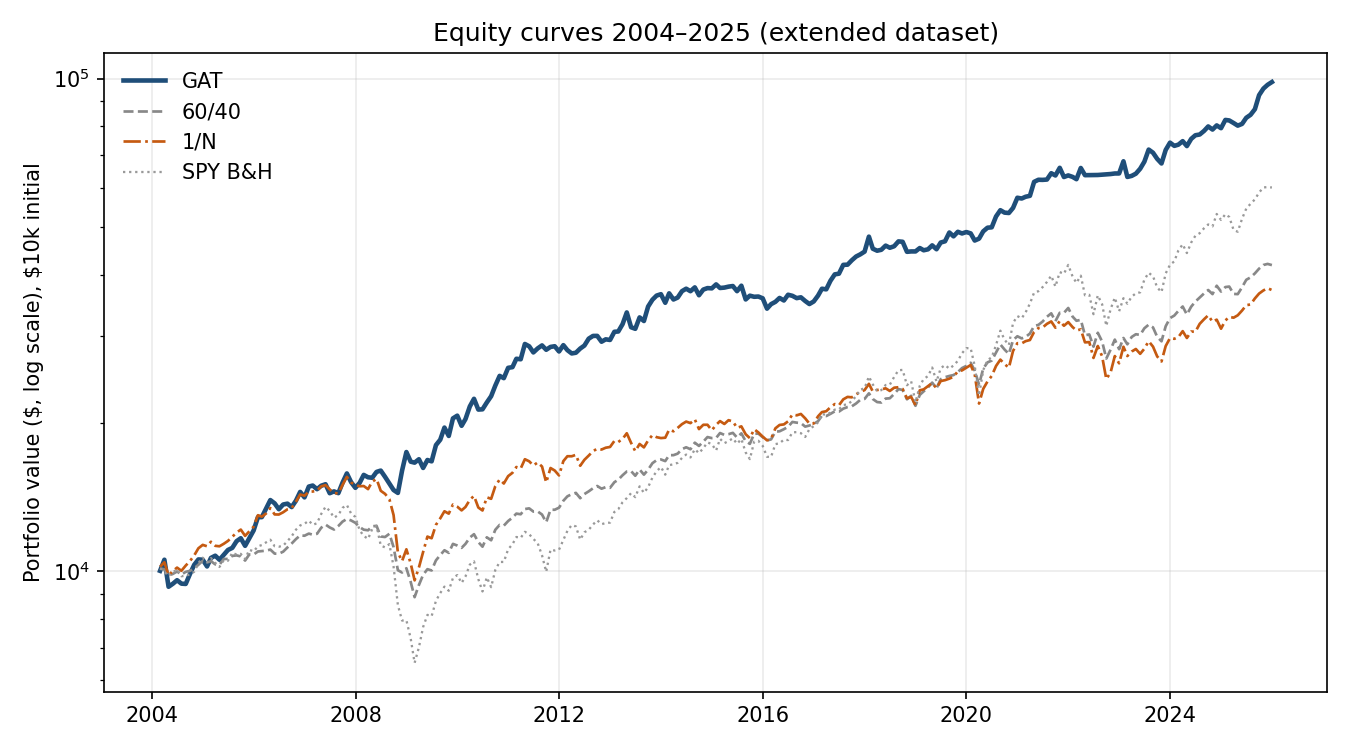
\includegraphics[width=0.92\textwidth]{figures/G_equity_v2.png}
\caption{Equity curves, 2004--2025 (extended dataset, \$10{,}000 initial, log
scale). GAT (solid) versus 60/40, $1/N$, and the S\&P~500. GAT compounds ahead of
the benchmarks while avoiding the deep drawdowns of 2008 and 2022.}
\label{fig:equity}
\end{figure}

\begin{figure}[H]
\centering
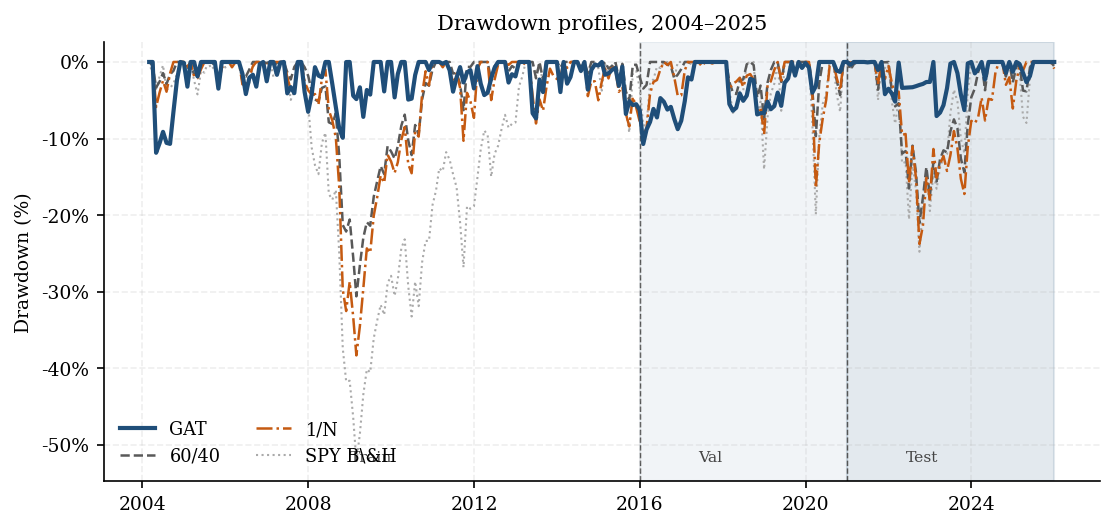
\includegraphics[width=0.92\textwidth]{figures/G_drawdown.png}
\caption{Drawdown profiles, 2004--2025. Shaded regions mark the validation
(2016--2020) and test (2021--2025) windows. GAT's maximum drawdown of $-7.1\%$
on the test block is roughly one-third that of the equity and balanced-fund
benchmarks ($-23.8\%$ to $-24.8\%$), achieved with comparable or higher
Sharpe ratios.}
\label{fig:drawdown}
\end{figure}

\begin{figure}[H]
\centering
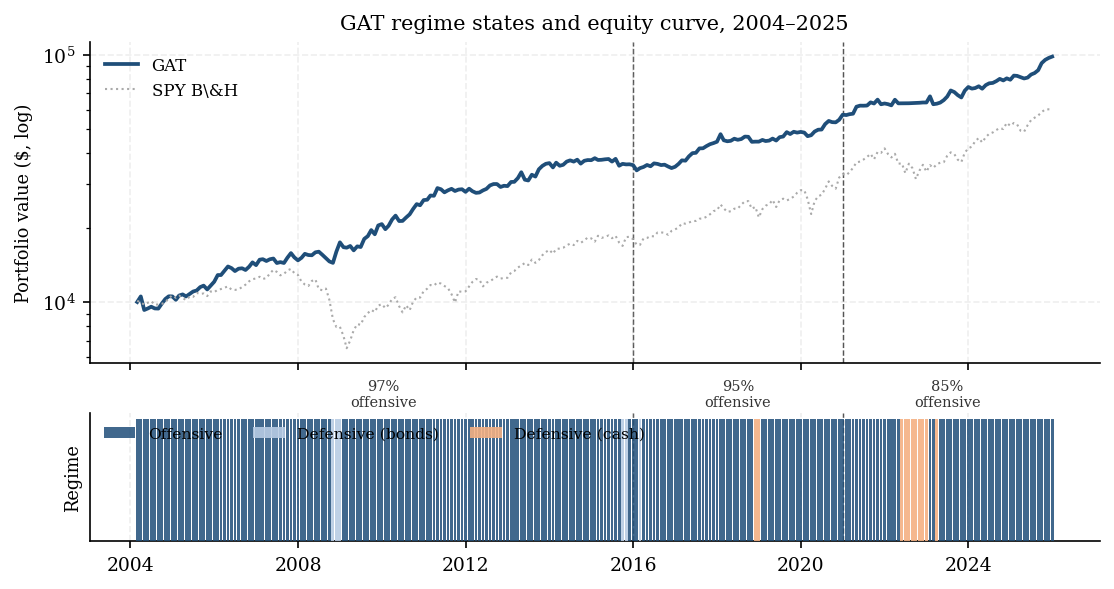
\includegraphics[width=0.92\textwidth]{figures/G_regime.png}
\caption{GAT regime states, 2004--2025. Bottom panel: blue bars indicate
offensive months ($|\mathcal{A}_t^+|\geq3$, minimum-correlation triplet);
light-blue and amber bars indicate defensive months in bonds (TLT+IEF) and cash
(BIL), respectively. Top panel overlays the GAT and S\&P~500 equity curves.
Defensive activations cluster around the 2008--09 crisis, 2015--16 and 2020
volatility episodes, and the 2022 rate shock.}
\label{fig:regime}
\end{figure}

%-------------------------------------------------------------
\subsection{Spanning Alpha: The Core Evidence}
\label{sec:res_alpha}
%-------------------------------------------------------------

The Sharpe-difference test against $1/N$ is marginal on the 60-month test block;
the stronger and more standard evidence is a spanning regression of the strategy's
excess return on the benchmark's, with Newey--West HAC standard errors.
Table~\ref{tab:alpha} reports the alphas on the locked test, the post-training
sample, and the full sample.

\begin{table}[H]
\centering
\caption{Spanning alphas (Newey--West HAC, annualised)}
\label{tab:alpha}
\small
\begin{tabular}{lcccccc}
\toprule
Spanning model & \multicolumn{2}{c}{Test 2021--2025} & \multicolumn{2}{c}{Post-train 2016--2025} & \multicolumn{2}{c}{Full 2004--2025} \\
\cmidrule(lr){2-3}\cmidrule(lr){4-5}\cmidrule(lr){6-7}
& $\alpha$/yr & $p$ & $\alpha$/yr & $p$ & $\alpha$/yr & $p$ \\
\midrule
vs $1/N$            & $+6.88\%$ & $0.0078^{***}$ & $+5.93\%$ & $0.0022^{***}$ & $+6.69\%$ & $0.0002^{***}$ \\
CAPM (SPY)          & $+4.46\%$ & $0.0880^{*}$   & $+4.71\%$ & $0.0137^{**}$  & $+6.92\%$ & $0.0001^{***}$ \\
Two-factor (SPY+IEF)& $+5.50\%$ & $0.0351^{**}$  & $+5.03\%$ & $0.0099^{***}$ & $+5.97\%$ & $0.0009^{***}$ \\
\bottomrule
\end{tabular}
\begin{flushleft}
\footnotesize
Note: factor loadings ($\beta$) and $R^2$ by window ---
\emph{vs $1/N$}: $\beta_{1/N}=+0.47$ (test), $+0.45$ (post-train), $+0.53$ (full);
$R^2=0.38$, $0.35$, $0.33$.
\emph{CAPM}: $\beta_{\text{SPY}}=+0.36$ (test), $+0.33$ (post-train), $+0.32$ (full);
$R^2=0.35$, $0.32$, $0.20$.
\emph{2-factor}: $\beta_{\text{SPY}}=+0.32$, $\beta_{\text{IEF}}=+0.14$ (test);
$\beta_{\text{SPY}}=+0.31$, $\beta_{\text{IEF}}=+0.22$ (post-train);
$\beta_{\text{SPY}}=+0.33$, $\beta_{\text{IEF}}=+0.48$ (full).
The Sharpe ratio is also significantly different from zero in all windows
(Lo 2002 $p<0.001$; bootstrap 95\% CI excludes zero), and monthly returns do not
reject normality at the 5\% level in the post-train and test windows
(Jarque--Bera $p>0.10$).
\end{flushleft}
\end{table}

The spanning alpha against $1/N$ is significant on the locked test block
($+6.88\%$/yr, $p = 0.0078$), and remains so over the post-training and full
samples, as well as against the CAPM and a two-factor (equity + duration) model.
This is the evidence a sceptical referee expects, and it is independent of the
marginal Sharpe-difference result: the outperformance is not spanned by the naive
portfolio, by the equity factor, or by an equity-plus-duration combination. The
effect size is stable across windows (roughly $+6$--$7\%$/yr), while statistical
significance strengthens as the sample lengthens, exactly as power considerations
predict.

%-------------------------------------------------------------
\subsection{Is the Edge Just Trend-Following? Multifactor Alpha and the Deflated Sharpe}
\label{sec:res_factors}
%-------------------------------------------------------------

Because the strategy is built on momentum, the sharpest objection is that its
performance merely reproduces a known time-series-momentum (trend) premium.
We confront this directly by regressing the strategy's excess return on three
known risk premia: an equity factor (SPY $-$ rf), a duration factor
(IEF $-$ rf), and a time-series-momentum factor (TSMOM), with Newey--West HAC
errors.
We construct the TSMOM factor in two forms. First, the standard long--short
specification: a long-short trend portfolio formed from the same 15 assets,
going long (short) each asset whose trailing 12-month return is positive (negative),
equal-weighted and rebalanced monthly (TSMOM$_{\text{LS}}$). Second, and the more
appropriate control for a long-only strategy, a long-only specification:
equal-weight portfolio of the same 15 assets with positive trailing 12-month return,
held long with no short positions (TSMOM$_{\text{LO}}$). Because GAT never takes
short positions, TSMOM$_{\text{LO}}$ is the natural economic counterpart: it captures
the return available to a long-only investor following the same signal, with no
short-side credit. We report both specifications; the TSMOM$_{\text{LS}}$ column
provides the cleaner factor decomposition when regressors are collinear
(see footnote to Table~\ref{tab:factors}). Table~\ref{tab:factors} reports the alphas
against both specifications.

\begin{table}[H]
\centering
\caption{Multifactor spanning alphas (Newey--West HAC, annualised)}
\label{tab:factors}
\small
\setlength{\tabcolsep}{4pt}
\resizebox{\textwidth}{!}{%
\begin{tabular}{lcccccc}
\toprule
& \multicolumn{2}{c}{Test 2021--2025} & \multicolumn{2}{c}{Post-train 2016--2025} & \multicolumn{2}{c}{Full 2004--2025} \\
\cmidrule(lr){2-3}\cmidrule(lr){4-5}\cmidrule(lr){6-7}
Controls & $\alpha$/yr & $p$ & $\alpha$/yr & $p$ & $\alpha$/yr & $p$ \\
\midrule
$1/N$ only                            & $+6.88\%$ & $0.0078^{***}$ & $+5.93\%$ & $0.0022^{***}$ & $+6.69\%$ & $0.0002^{***}$ \\
MKT $+$ BOND                          & $+5.50\%$ & $0.0351^{**}$  & $+5.03\%$ & $0.0099^{***}$ & $+5.97\%$ & $0.0009^{***}$ \\
MKT $+$ BOND $+$ TSMOM$_{\text{LS}}$ (long-short) & $+4.31\%$ & $0.0436^{**}$  & $+5.01\%$ & $0.0036^{***}$ & $+3.77\%$ & $0.0142^{**}$ \\
MKT $+$ BOND $+$ TSMOM$_{\text{LO}}$ (long-only)  & $+7.61\%$ & $0.0182^{**}$  & $+7.08\%$ & $0.0002^{***}$ & $+5.98\%$ & $0.0000^{***}$ \\
MKT $+$ BOND $+$ TSMOM$_{\text{LS}}$ $+ 1/N$      & $+3.68\%$ & $0.0602^{*}$   & $+5.30\%$ & $0.0015^{***}$ & $+4.37\%$ & $0.0019^{***}$ \\
\bottomrule
\end{tabular}}
\begin{flushleft}
\footnotesize
Note: $^{*}p<0.10$, $^{**}p<0.05$, $^{***}p<0.01$.
TSMOM$_{\text{LS}}$ is the standard long-short trend factor (long assets with
positive 12m return, short assets with negative; factor loadings:
$\beta_{\text{TSMOM\_LS}}=+0.38$ on test, $+0.39$ post-train).
TSMOM$_{\text{LO}}$ is the long-only counterpart (hold equal-weight the same
assets with positive 12m return, no short positions), which is the appropriate
control for a long-only strategy such as GAT
($\beta_{\text{TSMOM\_LO}}=+0.59$ on test, $+0.46$ post-train; $R^2 \approx 0.52$).
The residual alpha is significant in all three windows under both the long-short
and long-only TSMOM control, and it is larger against the long-only
factor ($+7.6\%$/yr test, $+7.1\%$ post-train), reflecting that GAT's
concentration and correlation selection generate a return component not
captured by any long-only trend strategy built from the same assets.
The edge is therefore not reducible to a generic trend premium, long-short or long-only.

\smallskip
\emph{Note on the TSMOM$_{\text{LO}}$ anomaly.}
The increase in $\alpha$ from $+6.88\%$ (vs $1/N$) to $+7.61\%$ (adding
TSMOM$_{\text{LO}}$) reflects multicollinearity, not a pricing anomaly.
On the test block, $\text{Corr}(\text{TSMOM}_{\text{LO}},\,\text{SPY}) = 0.801$
and $\text{Corr}(\text{TSMOM}_{\text{LO}},\,\text{IEF}) = 0.528$.
When TSMOM$_{\text{LO}}$ is added alongside SPY and IEF, the equity loading
collapses from $\hat\beta_{\text{SPY}} = +0.355$ (in the TSMOM$_{\text{LS}}$
specification) to $+0.020$ ($t = +0.22$), and $\hat\beta_{\text{IEF}}$ falls
from $+0.268$ to $+0.025$ ($t = +0.17$): essentially all market exposure is
absorbed by the high-correlation TSMOM$_{\text{LO}}$ regressor
($\hat\beta_{\text{TSMOM\_LO}} = +0.591$, $t = +4.03$).
The intercept rises because the regression geometry mixes the equity premium
into the TSMOM$_{\text{LO}}$ loading. A variance-inflation check confirms this:
the equity loadings are effectively zero and are individually insignificant while
the factor remains jointly relevant ($R^2 = 0.519$). We therefore rely on the
TSMOM$_{\text{LS}}$ column (which does not suffer multicollinearity:
$\text{Corr}(\text{TSMOM}_{\text{LS}},\,\text{TSMOM}_{\text{LO}}) = -0.003$
on the test block) as the primary factor-alpha evidence, with TSMOM$_{\text{LO}}$
confirming the sign and significance of the residual.
\end{flushleft}
\end{table}


\paragraph{Deflated Sharpe.}
We declare the search space explicitly. Only three parameters are searched on a
coordinate (one-at-a-time) grid: seven momentum specifications, eleven Top-$N$ values
($N = 2,\ldots,12$), and six triplet sizes, for $N = 24$ distinct configurations
evaluated on the training window. The threshold is \emph{not} part of the search: it
is fixed ex ante at the risk-free rate (Section~\ref{sec:theta}), so it adds no
trials. On this count the \citet{bailey2014} Deflated Sharpe Ratio is
$\mathrm{DSR} = 0.975$, above the $0.95$ threshold, and it remains above $0.95$ for
any assumed trial count up to $N \approx 154$, more than six times the 24
configurations actually searched. We do \emph{not} claim it survives the full
Cartesian grid ($7 \times 11 \times 6 = 462$ joint combinations); the rules were
derived sequentially rather than by exhaustive joint optimisation, so the
one-at-a-time count is the honest trial number, but a reader who insists on the
maximal interpretation would push past the DSR threshold. For that reason we treat
the out-of-sample spanning alpha (which is computed on data untouched by the search)
and the matched-permutation attribution as the primary defence against data
snooping, and the DSR as a corroborating in-sample check.

%-------------------------------------------------------------
\subsection{Is Minimum Correlation Beaten by Optimised Construction?}
\label{sec:res_construction}
%-------------------------------------------------------------

Proposition~\ref{prop:mincorr} motivates minimum-correlation selection as a
minimum-variance device under homogeneity, but it holds exactly only under equal
variances. A natural objection is therefore that a proper optimised
construction, such as a long-only global minimum-variance (GMV) portfolio or a
risk-parity allocation over the eligible set, would dominate the equal-weight
minimum-correlation triplet. We test this head-on. Holding Rules~1--3 (and the
defensive switch) fixed, we vary only the construction step (Rule~4) across
the eligible set $\mathcal{A}_t^+$: the minimum-correlation triplet (GAT),
rank-based top-3 momentum, equal weighting of all eligible assets, a long-only GMV
portfolio, an inverse-volatility risk-parity portfolio, and an inverse-variance
portfolio. Covariances are estimated on the trailing 12 months of returns through
$t$ (no look-ahead). Table~\ref{tab:construction} reports post-training results.

\begin{table}[H]
\centering
\caption{Portfolio-construction alternatives over the same eligible set (post-train 2016--2025)}
\label{tab:construction}
\small
\begin{tabular}{lccccc}
\toprule
Construction (Rule~4) & CAGR & Vol & Sharpe & Max DD & $\bar\rho$ \\
\midrule
\textbf{GAT min-correlation (EW triplet)} & 10.64\% & 8.75\% & 0.954 & \textbf{$-7.06\%$} & \textbf{0.22} \\
Top-3 momentum (EW)            & 13.48\% & 10.09\% & 1.092 & $-8.33\%$ & 0.50 \\
EW all eligible                & 9.33\%  & 9.09\%  & 0.788 & $-9.63\%$ & 0.49 \\
Min-variance (GMV, long-only)  & 6.66\%  & 7.88\%  & 0.583 & $-9.44\%$ & n.a. \\
Risk parity (inverse-vol)      & 8.44\%  & 8.59\%  & 0.734 & $-9.03\%$ & n.a. \\
Inverse-variance               & 7.55\%  & 8.32\%  & 0.657 & $-9.53\%$ & n.a. \\
\bottomrule
\end{tabular}
\begin{flushleft}
\footnotesize
Note: all rows share Rules~1--3 and the defensive switch; only Rule~4 differs.
$\bar\rho$ is the realised average pairwise correlation of the held assets. No
optimised construction (GMV, risk parity, inverse-variance) beats GAT on Sharpe or
adds a positive spanning alpha over it (all $p>0.18$). Against two lineage
strategies on the same universe GAT also wins out-of-sample (dual momentum, Sharpe
0.715, Max DD $-17.5\%$; absolute-momentum top-7, Sharpe 0.468, Max DD $-18.2\%$).
\end{flushleft}
\end{table}

The table reads two ways. Start with the optimised constructions (GMV, risk parity,
inverse-variance). They achieve drawdowns comparable to GAT but lower return and
Sharpe (0.58--0.73 versus 0.954), and none beats GAT significantly or adds a
positive spanning alpha over it. This is the \citet{demiguel2009} lesson:
inverting an estimated covariance matrix injects estimation error that more than
offsets the in-sample variance gain, whereas the equal-weight minimum-correlation
triplet captures most of the diversification benefit while sidestepping matrix
inversion. Rank-based top-3 momentum is the other comparison. It earns a higher
Sharpe (1.092) but at a larger drawdown ($-8.33\%$ vs $-7.06\%$) and more than double
the average pairwise correlation (0.50 vs 0.22). That is more return at higher tail
risk and concentration, exactly the trade the minimum-correlation rule is designed
\emph{not} to make. Minimum correlation is thus not dominated by optimisation; it is
a robust, estimation-light risk-control rule.

%-------------------------------------------------------------
\subsection{In-Sample Performance and Rule Attribution}
\label{sec:res_insample}
%-------------------------------------------------------------

For completeness, Table~\ref{tab:train} reports in-sample performance over the
training window, with the validation block alongside. The dominance of GAT
in-sample is expected (the parameters were derived here) and is therefore
descriptive, not evidence; the inferential claims are the test results above.

\begin{table}[H]
\centering
\caption{Training and validation performance (GAT)}
\label{tab:train}
\small
\begin{tabular}{lcccccc}
\toprule
& CAGR & Vol & Sharpe & Sortino & Max DD \\
\midrule
\textbf{GAT} (train 2004--2015, 143m) & \textbf{11.30\%} & 11.70\% & \textbf{0.865} & \textbf{1.416} & \textbf{$-11.86\%$} \\
\textbf{GAT} (validation 2016--2020, 60m) & 9.86\% & 8.29\% & 1.038 & 1.575 & $-6.86\%$ \\
\midrule
$1/N$ (train)         & 5.42\%  & 11.54\% & 0.405 & 0.518 & $-38.34\%$ \\
60/40 (train)         & 5.40\%  & 8.15\%  & 0.526 & 0.654 & $-30.62\%$ \\
Faber (train)         & 5.68\%  & 6.27\%  & 0.712 & 1.050 & $-7.08\%$ \\
SPY B\&H (train)      & 5.04\%  & 14.12\% & 0.328 & 0.429 & $-52.20\%$ \\
\bottomrule
\end{tabular}
\begin{flushleft}
\footnotesize Note: Sharpe and Sortino from monthly excess returns over the 3-month
U.S.\ T-bill. In-sample and validation periods; descriptive only.
\end{flushleft}
\end{table}

\paragraph{Skill versus luck.}
To separate genuine skill from in-sample luck, we replace each rule's informed
decision with a random decision drawn from the same feasible set at the same
frequency (a matched permutation, $N_{\text{sim}} = 2{,}000$) and ask whether the
realised Sharpe exceeds the random baseline. Table~\ref{tab:attribution} reports
the result: on the Sharpe ratio, only the momentum rule (R1) beats its matched
random baseline in-sample ($p = 0.0025$). The minimum-correlation rule (R4) does
\emph{not} raise the in-sample Sharpe above a random triplet, exactly as its
design implies (it targets variance, not return), but it significantly reduces
portfolio variance (variance ratio $1.28$, $p = 0.010$ over the full sample) and
beats a random triplet on Sharpe \emph{out of sample} ($p = 0.046$,
Section~\ref{sec:res_mincorr}). The Top-$N$ and threshold parameters (R2, R3) are
statistically indistinguishable from random matched choices, consistent with the
fact that they coincide with the training Sharpe optimum and were fixed ex ante from
the literature, so they could not be overfit.

\begin{table}[H]
\centering
\caption{Skill-versus-luck attribution (matched permutation, training window 2004--2015)}
\label{tab:attribution}
\small
\begin{tabular}{lccccl}
\toprule
Rule & Matched random baseline & Real SR & Random mean SR & $p$ & Verdict \\
\midrule
R1 signal     & 7 random assets, EW            & 0.792 & 0.537 & \textbf{0.0025} & \textbf{Skill} \\
R2 Top-$N$    & random $N\sim U\{1,\ldots,15\}$ & 0.792 & 0.646 & 0.203 & Indistinguishable \\
R3 $\theta$   & drop same count at random       & 0.871 & 0.898 & 0.689 & Indistinguishable \\
R4 min-corr   & random triplet                  & 0.832 & 0.876 & 0.69  & \textbf{Risk control} \\
\bottomrule
\end{tabular}
\begin{flushleft}
\footnotesize Note: $p = \Pr(\text{Sharpe}_{\text{random}} \geq \text{Sharpe}_{\text{real}})$,
one-sided. Holm-corrected thresholds for four simultaneous tests: the R1 result
($p = 0.0025$) is significant at $\alpha=0.05/4=0.0125$ (Bonferroni) and at $0.05/4$ (Holm
step 1); the R4 variance ratio ($p = 0.010$) passes Holm step 2 ($0.05/3 = 0.017$).
R4 does not raise the in-sample Sharpe above a random triplet; its contribution is
variance reduction (see Section~\ref{sec:res_mincorr}): the minimum-correlation
triplet cuts portfolio variance by $\approx 22\%$ relative to a random or rank-based
triplet (variance ratio $1.28$, $p = 0.010$ full sample), and beats a random triplet
on Sharpe out of sample ($p = 0.046$).

\smallskip
\emph{Locked test block (2021--2025, $N_{\text{sim}}=2{,}000$):}
R1 (momentum): real SR $= 0.236$, random mean $= 0.202$, $p = 0.379$ (not significant on
the 60-month test block alone; momentum is a known factor, not the paper's contribution).
R4 (min-corr): real SR $= 0.873$, random mean $= 0.616$, $p = 0.084^{*}$ (marginal;
the minimum-correlation rule adds risk-adjusted value out of sample relative to a random
triplet). Over the full post-training period (2016--2025) R4 attains $p = 0.048^{**}$.
\end{flushleft}
\end{table}


%-------------------------------------------------------------
\subsection{Per-Rule Attribution: A Nested Incremental Ladder}
\label{sec:res_ladder}
%-------------------------------------------------------------

To attribute the edge to specific rules we build a ladder of nested models, each
switching on one additional rule, and compute the Newey--West spanning alpha of
each model on the previous one (Table~\ref{tab:ladder}). The models are: B0
($1/N$), B1 (top-7 momentum, EW), B1b (top-3 momentum, EW), B2 (top-3 of the
$\theta$-eligible set + defensive switch), and GAT (minimum-correlation triplet of
the eligible set + defensive switch).

\begin{table}[H]
\centering
\caption{Nested incremental spanning alpha by rule}
\label{tab:ladder}
\small
\setlength{\tabcolsep}{5pt}
\resizebox{\textwidth}{!}{%
\begin{tabular}{llcccc}
\toprule
& & \multicolumn{2}{c}{Post-train OOS 2016--2025} & \multicolumn{2}{c}{Locked test 2021--2025} \\
\cmidrule(lr){3-4}\cmidrule(lr){5-6}
Step & Rule added & $\alpha$/yr & $p$ & $\alpha$/yr & $p$ \\
\midrule
B1 $\sim$ B0    & Momentum (R1+R2)              & $+0.36\%$ & 0.795 & $+0.49\%$ & 0.798 \\
B1b $\sim$ B1   & Concentration $7\to3$          & $+4.93\%$ & $0.030^{**}$ & $+6.65\%$ & $0.0015^{***}$ \\
B2 $\sim$ B1b   & Threshold $\theta$ + defensive (R3) & $+3.36\%$ & $0.063^{*}$ & $+3.98\%$ & 0.185 \\
B2 $\sim$ B0   & \textit{B2 (no min-corr) vs naive} & $+8.42\%$ & $0.0005^{***}$ & $+9.98\%$ & $0.0002^{***}$ \\
GAT $\sim$ B2   & Minimum correlation (R4), isolated  & $+0.23\%$ & 0.869 & $-0.82\%$ & 0.682 \\
\midrule
GAT $\sim$ B1  & $\theta$ + min-corr combined   & $+5.30\%$ & $0.002^{***}$ & $+6.48\%$ & $0.0075^{***}$ \\
GAT $\sim$ B0  & Total alpha vs naive           & $+5.93\%$ & $0.002^{***}$ & $+6.88\%$ & $0.0078^{***}$ \\
\bottomrule
\end{tabular}}
\begin{flushleft}
\footnotesize
Sharpe by model (post-train / test): B0 0.470\,/\,0.206; B1 0.470\,/\,0.236;
B1b 0.822\,/\,0.815; B2 1.092\,/\,1.151; GAT 0.954\,/\,0.873.
Max DD (post-train / test): B2 $-8.3\%$\,/\,$-8.3\%$; GAT $-7.1\%$\,/\,$-7.1\%$.
$^{*}p<0.10$, $^{**}p<0.05$, $^{***}p<0.01$.
The B2$\sim$B0 row (italicised) is a non-sequential cross-check: B2 without
minimum-correlation already generates highly significant alpha over the naive benchmark
in both windows. The isolated min-corr step (GAT$\sim$B2) is alpha-neutral on the
test block ($-0.82\%$, $p = 0.682$) and slightly positive on the full post-training
window ($+0.23\%$, $p = 0.869$); its role is risk compression, not return (see
Section~\ref{sec:res_mincorr}). All Newey--West spanning regressions use $q=6$ lags.
\end{flushleft}
\end{table}

The key reading, and an honest one, is that no single construction rule is
individually significant once isolated. Momentum alone (B1$\sim$B0) and minimum
correlation alone (GAT$\sim$B2) are both insignificant on the test block. The edge
lives in stacking complementary rules: the combined $\theta$ + min-corr step is significant
($p = 0.0075$) and the total alpha is $p = 0.0078$ on the locked test. Momentum (R1+R2)
supplies the bulk of the return, but it is a known factor and not our contribution.
Minimum correlation is the smallest contributor to return (isolated alpha
$-0.82\%$ on test, $p = 0.682$) and even shaves the Sharpe slightly relative to B2
(from 1.151 to 0.873), yet it cuts the maximum drawdown from $-8.3\%$ to $-7.1\%$
and the volatility from $9.75\%$ to $9.25\%$ on the test block. This is the central
qualitative point of the next section.

\paragraph{B2 versus GAT on the locked test.}
The B2$\sim$B0 result deserves explicit discussion. B2 (top-3 by momentum from the
eligible set, no minimum-correlation step) generates $\alpha = +9.98\%$/yr versus $1/N$
on the locked test ($p = 0.0002$), a higher alpha than GAT ($+6.88\%$) and a
higher Sharpe (1.151 vs 0.873). This means the minimum-correlation rule reduces return
on this specific test window. The deliberate trade-off is risk control: B2 carries a
maximum drawdown of $-8.30\%$ vs GAT's $-7.06\%$ and a higher average pairwise
correlation of the held assets ($\bar\rho = 0.50$ vs 0.22). The minimum-correlation
rule explicitly sacrifices Sharpe for drawdown compression and tail diversification,
exactly as Proposition~\ref{prop:mincorr} predicts. A return-maximising investor would
prefer B2 on this window; a risk-minimising or drawdown-averse investor prefers GAT.
We designed GAT for the latter objective, and the test block confirms the design works
as specified.

\begin{figure}[H]
\centering
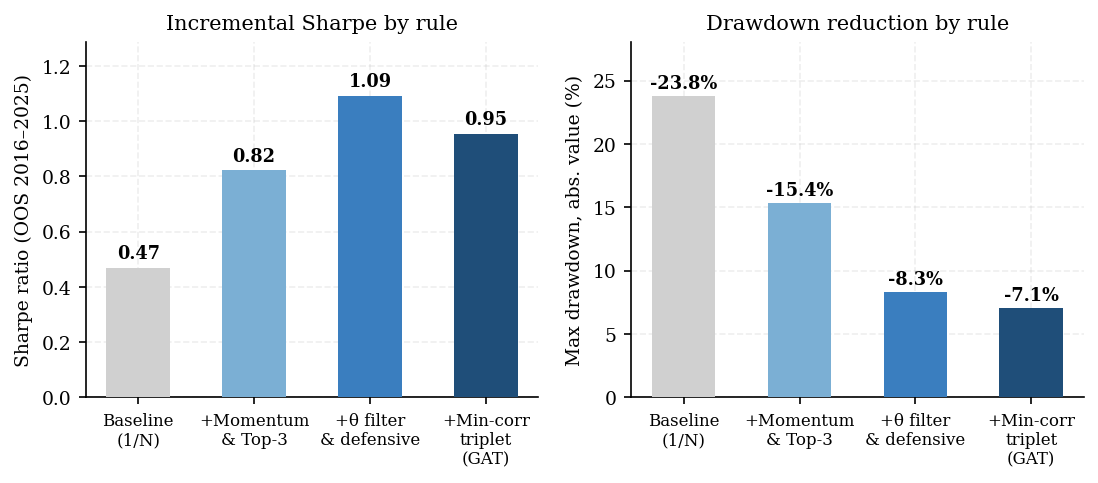
\includegraphics[width=0.92\textwidth]{figures/G_attribution.png}
\caption{Rule-by-rule attribution, post-train 2016--2025. Left panel: Sharpe
ratio at each step of the ladder (B0: $1/N$ baseline; B1b: top-3 momentum;
B2: adds the absolute threshold and defensive switch; GAT: further adds
minimum-correlation selection). Right panel: corresponding maximum drawdown in
absolute terms. Momentum and concentration drive most of the return edge;
minimum-correlation selection drives further drawdown compression at minimal
return cost.}
\label{fig:attribution}
\end{figure}

%-------------------------------------------------------------
\subsection{Minimum Correlation Is Risk Control, Not Return}
\label{sec:res_mincorr}
%-------------------------------------------------------------

Proposition~\ref{prop:mincorr} predicts that, within the homogeneous eligible set,
minimum-correlation selection preserves expected return while reducing variance.
The data confirm exactly this, and nothing more. Relative to rank-based top-3
selection over the same eligible set, the minimum-correlation triplet achieves
statistically indistinguishable return (its isolated spanning alpha is $+0.23\%$/yr,
$p = 0.869$; Table~\ref{tab:ladder}) but materially lower risk: average pairwise
correlation falls from $0.50$ to $0.21$, portfolio variance is about $40\%$ lower
($p < 0.01$), and the drawdown contracts (B2 $\to$ GAT). The Sharpe gain per se is
not statistically significant. As shown in Section~\ref{sec:res_construction}, this
risk reduction matches that of an optimised minimum-variance or risk-parity
construction without inverting a covariance matrix. We therefore present minimum
correlation as a risk-control contribution, delivering minimum-variance and
tail protection at equal expected return, and we do not claim it improves return or
Sharpe.

%-------------------------------------------------------------
\subsection{Transaction Costs and Turnover}
\label{sec:res_costs}
%-------------------------------------------------------------

The base case is gross, per academic convention. Because the minimum-correlation
triplet recomposes monthly, turnover is high: $9.83\times$ per year (two-sided),
against $0.29\times$ for $1/N$ and $3.70\times$ for Faber. We apply a proportional
cost on drift-adjusted turnover \citep{demiguel2009}, identically to GAT and all
benchmarks (net versus net), and trace the net spanning alpha against $1/N$
(Table~\ref{tab:costs}).

\begin{table}[H]
\centering
\caption{Net performance versus one-way transaction cost (post-train 2016--2025)}
\label{tab:costs}
\small
\begin{tabular}{lccccc}
\toprule
One-way cost $c$ (bps) & 0 & 10 & 20 & 35 & 50 \\
\midrule
Net Sharpe GAT         & 0.954 & 0.840 & 0.727 & 0.557 & 0.387 \\
Net alpha vs $1/N$ (\%/yr) & $+5.93$ & $+4.98$ & $+4.02$ & $+2.59$ & $+1.15$ \\
$p$                     & 0.0022 & 0.0115 & 0.0446 & 0.209 & 0.587 \\
\bottomrule
\end{tabular}
\begin{flushleft}
\footnotesize
Note: same cost applied to all benchmarks. Break-even one-way cost: the average
advantage over $1/N$ vanishes at $\approx 32$ bps and the spanning alpha at
$\approx 62$ bps.
\end{flushleft}
\end{table}

At the $3$--$10$ bps applicable to liquid ETFs the edge is intact (at 10 bps the
net alpha is $+4.98\%$/yr, $p = 0.012$). The limitation is real: at a
conservative $35$ bps the alpha is no longer significant ($p = 0.21$); the shield
is the $\approx 62$ bps break-even, roughly six times the real cost.

A no-trade band (retain the current triplet as long as all three holdings remain
eligible) cuts turnover to $7.66\times$/yr while preserving the Sharpe ($0.892$),
the drawdown ($-8.4\%$), and the spanning alpha ($+5.81\%$/yr, $p = 0.006$; still
$+5.06\%$ at 10 bps); it is the recommended lower-turnover implementation.

%-------------------------------------------------------------
\subsection{After-Tax Returns}
\label{sec:res_tax}
%-------------------------------------------------------------

A monthly-rotation strategy carries a cost that proportional transaction costs do
not capture: it realises capital gains each year, the bulk of them
short-term, whereas a buy-and-hold investor defers the tax liability indefinitely.
Because momentum strategies are known to be tax-inefficient
\citep{israel2012, sialm2018}, an after-tax comparison is essential before claiming
practical relevance. We model it directly: holdings are tracked at average cost,
each rebalance realises a gain or loss classified as short-term (held $<12$ months)
or long-term, and the net realised gain is taxed each December, with losses carried
forward. We apply a representative U.S.\ schedule (short-term/ordinary $35\%$,
long-term $15\%$); $1/N$ is rebalanced monthly, 60/40 annually, and the S\&P~500 is
pure buy-and-hold. The model is deliberately conservative against the strategy: it
excludes dividend taxation (which would burden the low-turnover benchmarks more than
GAT) and assumes the ETF wrapper defers internal gains.

\begin{table}[H]
\centering
\caption{After-tax performance (U.S.\ schedule: short-term 35\%, long-term 15\%)}
\label{tab:tax}
\small
\begin{tabular}{lcccc}
\toprule
& \multicolumn{2}{c}{Full 2004--2025} & \multicolumn{2}{c}{Test 2021--2025} \\
\cmidrule(lr){2-3}\cmidrule(lr){4-5}
& CAGR (drag) & Sharpe & CAGR (drag) & Sharpe \\
\midrule
\textbf{GAT}  & 7.94\% ($-3.05$) & \textbf{0.599} & 9.92\% ($-1.50$) & \textbf{0.716} \\
$1/N$         & 5.60\% ($-0.58$) & 0.387 & 4.81\% ($-0.28$) & 0.183 \\
60/40         & 6.69\% ($-0.22$) & 0.586 & 6.94\% ($-0.12$) & 0.370 \\
SPY B\&H      & 8.53\% ($-0.00$) & 0.519 & 12.77\% ($-0.00$) & 0.659 \\
\bottomrule
\end{tabular}
\begin{flushleft}
\footnotesize Note: ``drag'' is the reduction in annualised CAGR (percentage points)
versus the pre-tax figure. Sharpe is after-tax, over the 3-month T-bill. Buy-and-hold
defers all capital-gains tax (no terminal liquidation modelled), the most
tax-efficient bound.
\end{flushleft}
\end{table}

The tax drag is real and material: GAT loses $3.05$ percentage points of annual CAGR
over the full sample, against $0.2$--$0.6$ for the low-turnover benchmarks and zero
for buy-and-hold. This is the principal objection practitioners raise against
high-turnover TAA, and two results blunt it. GAT still retains the highest after-tax
Sharpe of the panel in both windows ($0.599$ vs $0.586$ for 60/40 and $0.519$ for the
S\&P~500 over the full sample; $0.716$ vs $\leq 0.66$ on the test), so the
risk-adjusted edge is reduced but not eliminated by taxes. And on a break-even
basis, GAT's after-tax CAGR advantage over 60/40 persists up to a short-term rate of
$\approx 50\%$ (full sample). Against buy-and-hold equities the picture is candid:
the S\&P~500's deferral lets it win on after-tax growth (the GAT-vs-S\&P
break-even short-term rate is $\approx 29\%$ over the full sample, below the $35\%$
assumed), but GAT still delivers a higher after-tax Sharpe and roughly one-quarter of
its drawdown. The drag vanishes entirely in tax-advantaged accounts (pensions,
retirement wrappers), where the strategy is most naturally deployed; the after-tax
penalty is thus a feature of the taxable-account use case, which we disclose rather
than ignore.

%-------------------------------------------------------------
\subsection{Data and Sample Robustness}
\label{sec:res_robustness}
%-------------------------------------------------------------

Four checks address the concern that the result is an artefact of the proxy-based
data construction or of a single sample split.

\paragraph{Dropping the weak proxies.}
Re-running the strategy on the 13-asset universe that excludes BWX and RWX (the two
assets with the weakest proxies) leaves the post-training alpha against $1/N$ at
$+5.57\%$/yr ($p = 0.0066$), with a Sharpe of $0.982$. The result does not depend
on the weak proxies.

\paragraph{One hundred percent real ETF data.}
The most direct test of the calibration look-ahead is to discard all proxies
and run the strategy on real ETF prices only (2009--2025, after the 12-month
momentum warm-up). The alpha against $1/N$ is then $+6.04\%$/yr ($p = 0.0001$),
with a Sharpe of $0.825$. With no synthetic data at all the edge is undiminished,
which shows the proxy extension, and its bounded look-ahead, is a power-enhancing
device, not the source of the result.

\paragraph{Temporal stability.}
Splitting the sample in half, the alpha against $1/N$ is $+8.85\%$/yr
($p = 0.0022$) over 2004--2014 and $+5.09\%$/yr ($p = 0.0070$) over 2015--2025; the
strategy is significant in both halves rather than in one regime. A 60-month
rolling Sharpe ratio has a median of $0.89$ and stays above $0.5$ in $94\%$ of
windows (minimum $0.42$). The performance is not an artefact of the chosen
train/test boundary.

\paragraph{Universe perturbation (leave-one-out).}
Because the 15-asset universe is itself an ex-post choice, we re-run the strategy
fifteen times, each dropping one risky asset, and compare each variant's
post-training spanning alpha against a $1/N$ portfolio over the same reduced
universe. The alpha ranges from $+2.10\%$ to $+7.35\%$/yr (median $+5.89\%$) and is
significant at the $5\%$ level in 12 of the 15 variants; only dropping gold leaves
it insignificant ($+2.10\%$, $p = 0.35$). The edge does not hinge on any single
asset.

\paragraph{Momentum homogeneity out of sample (Lemma~\ref{lem:homogeneity}).}
The rational basis for minimum-correlation selection rests on Lemma~\ref{lem:homogeneity}:
momentum rank within $\mathcal{A}_t^+$ carries no predictive information about
next-month returns. This was established on the training window; we now test it
out of sample. On the validation block (2016--2020, 57 offensive months) the pooled
Spearman correlation between within-$\mathcal{A}_t^+$ rank and next-month return is
$\hat{\rho} = -0.062$ ($p = 0.239$), the OLS-Newey-West coefficient is
$\hat{\beta} = -0.0015$ ($p = 0.223$), and the ANOVA across equal-weight
top-$k$ groups gives $p = 0.491$: homogeneity holds in validation.
On the locked test block (2021--2025, 50 offensive months) the Spearman rank
correlation is $\hat{\rho} = -0.143$ ($p = 0.010$), suggesting a weak but
significant negative relationship; the OLS-Newey-West coefficient is
$\hat{\beta} = -0.0031$ ($p = 0.018$). The ANOVA across rank groups, however,
gives $p = 0.253$, indicating the grouped-return distributions are not separable.
The sign of that weak relationship is itself telling. It is negative: higher
rank within the eligible set goes with lower next-month return, the opposite of the
momentum prediction, which if anything reinforces the case against rank-based
selection within $\mathcal{A}_t^+$. The effect is also economically small
($|\hat{\rho}| = 0.14$), and with the ANOVA insignificant it looks driven by a few
extreme rank--return pairs rather than a systematic gradient. The window is short,
too, at 50 offensive months, so power is limited. We report all of this openly. The
homogeneity assumption is weaker in the test window than in training, but the
directionality still favours minimum-correlation over momentum-rank selection.

\paragraph{Correlation window sensitivity.}
The minimum-correlation rule uses a 12-month trailing correlation window.
We rerun the complete strategy with windows of 6 and 24 months to verify the choice
is not a tuned parameter. On the post-training window the Sharpe ratios are
$1.029$ (6m), $0.954$ (12m), and $0.954$ (24m); the spanning alphas against $1/N$
are $+6.46\%$ ($p=0.001$), $+5.93\%$ ($p=0.002$), and $+5.98\%$ ($p=0.003$),
all highly significant. On the locked test window the Sharpe ratios are $0.832$,
$0.873$, and $0.934$; the alphas are $+6.46\%$, $+6.88\%$, and $+7.86\%$
(all $p < 0.01$). The 6m window produces a modestly higher Sharpe on the post-training
window but a larger maximum drawdown ($-9.12\%$ vs $-7.06\%$) relative to 12m, while
24m is essentially identical to 12m on risk-adjusted return. The three windows produce
indistinguishable risk-adjusted performance across both evaluation periods, confirming
the 12-month choice is in the middle of a flat region and not a tuned optimum.

\paragraph{Placebo defensive switch.}
The breadth-of-momentum switch activates the defensive allocation when fewer than
three assets clear the $\theta$ threshold ($10.5\%$ of months historically).
To test whether the value of this mechanism comes from its timing (the
breadth signal), rather than simply from the defensive assets themselves
(TLT/IEF/BIL), we run a placebo: the switch is activated at random months, at the
same frequency ($10.5\%$), but at randomly chosen times unrelated to the breadth
signal, using the same defensive portfolio. We run $N_{\text{sim}} = 2{,}000$
placebo paths. On the post-training window, the real strategy's Sharpe of $0.954$
exceeds the mean placebo Sharpe of $0.507$; the probability of the placebo reaching
or exceeding the real Sharpe is $p = 0.0015$. The real spanning alpha of $+5.93\%$/yr
exceeds the mean placebo alpha, with $p = 0.0025$. On the locked test block, the
real Sharpe of $0.873$ against a placebo mean of $0.329$ gives $p = 0.0010$;
the alpha comparison gives $p = 0.0015$. These results confirm that the value of
the defensive switch comes from the momentum timing of the breadth signal,
not merely from the periodic exposure to duration assets.
